\documentclass[a4paper, 12pt]{article}
\usepackage[spanish]{babel}
\usepackage[hmargin=2cm,vmargin=2.5cm]{geometry}
\usepackage{enumerate}
\usepackage{makecell}
\usepackage{graphicx}
\usepackage{hyperref}
\usepackage{amsmath}
\usepackage[backend=biber,style=apa, url=true, sortcites]{biblatex}
\usepackage[table]{xcolor}
\usepackage{minted}
\usepackage{graphicx}
\usepackage{fancyhdr}  % Agrega el paquete fancyhdr
\usepackage{subcaption}

\addbibresource{references.bib}
\hypersetup{
	colorlinks,
	citecolor=black,
	filecolor=black,
	linkcolor=black,
	urlcolor=black
}

\setlength{\arrayrulewidth}{0.4mm}

\newcommand{\HRule}{\rule{\linewidth}{0.5mm}}

\begin{document}
	\begin{titlepage}
		\begin{center}
			% logo
			
\includegraphics[width=0.5\textwidth]{figures/logoUAH.png}~\\[2cm]
			
			\textsc{\Large \\Sistemas de Control Inteligente}\\[2cm]
			
			\HRule \\[0.4cm]
			{\LARGE \bfseries Práctica 0 \\ Introducción a Matlab (I) \\[0.4cm]}
			\HRule \\[3cm]
			
			\large\textbf{Jorge Revenga Martín de Vidales}\\
			\large\textbf{Ángel Salgado}\\
			\large\textbf{}\\ Grado en Ingeniería Informática \\ Universidad de Alcalá
			
			\vfill
			
			{\large \today}
		\end{center}
	\end{titlepage}
	
	% Configura los encabezados y pies de página
	\pagestyle{fancy}
	\fancyhf{} % Limpia todos los encabezados y pies de página actuales
	% Encabezado
	\fancyhead[RO,LE]{\textit{Sistemas de Control Inteligente}}
	\fancyhead[LO,RE]{\textit{Ejercicios de Introducción a Matlab (I)}}  % Título del documento
	% Pie de página
	\fancyfoot[LO,RE]{\textit{Universidad de Alcalá}}
	\fancyfoot[RO,LE]{\thepage}  % Número de página en la esquina inferior derecha
	\newpage
	
	\thispagestyle{plain}
	\tableofcontents
	\newpage
	
	\section{Ejercicio 1. Matrices y vectores.}
	
	\subsection{Código}
	\inputminted[fontsize=\scriptsize, linenos, breaklines=true, xleftmargin=0.75cm, frame=lines]{matlab}{code/Ejercicio1.m}
	\subsection{Ejecución}
	\begin{figure}[htp!]
		\centering
		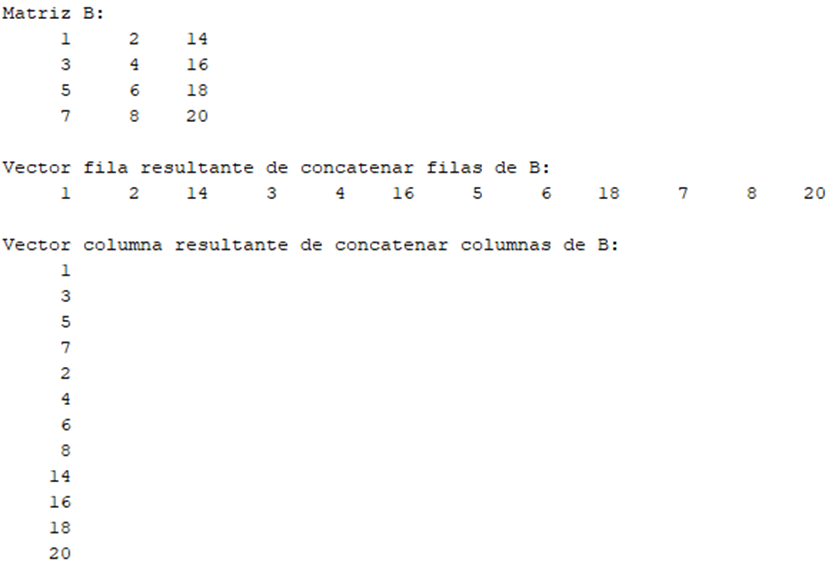
\includegraphics[width=0.7\textwidth]{figures/ejc1.png}
		\caption{Ejecución ejercicio 1.}
	\end{figure}
	
	\section{Ejercicio 2. Matrices y vectores.}
	
	\subsection{Código}
	\inputminted[fontsize=\scriptsize, linenos, breaklines=true, xleftmargin=0.75cm, frame=lines]{matlab}{code/Ejercicio2.m}
	\subsection{Ejecución}
	\begin{figure}[htp!]
		\centering
		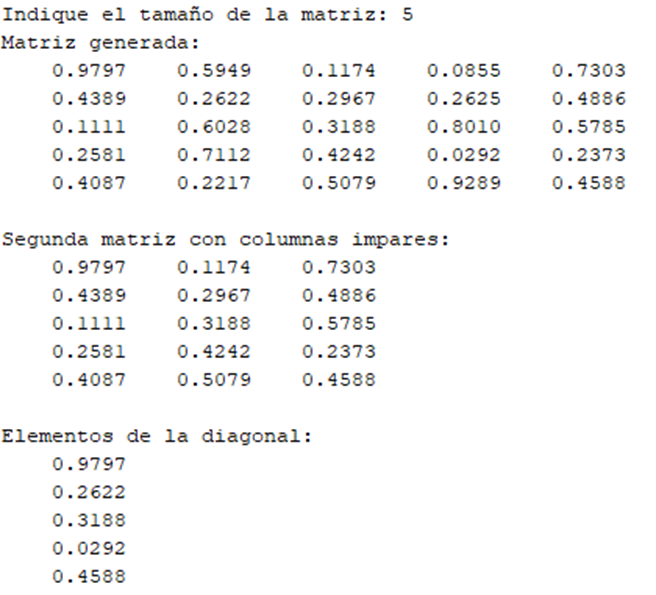
\includegraphics[width=0.6\textwidth]{figures/ejc2.png}
		\caption{Ejecución ejercicio 2.}
	\end{figure}
	\begin{figure}[htp!]
		\centering
		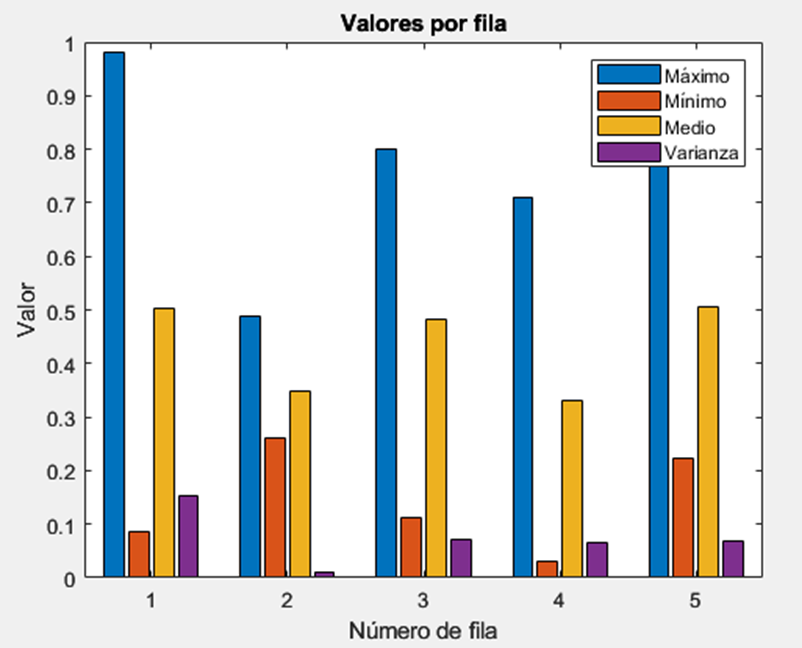
\includegraphics[width=0.6\textwidth]{figures/graf1.png}
		\caption{Gráfico ejecución ejercicio 2.}
	\end{figure}
	
	\section{Ejercicio 3. Matrices y vectores.}
	
	\subsection{Código}
	\subsubsection*{IntroducirMatriz.m}
	\inputminted[fontsize=\scriptsize, linenos, breaklines=true, xleftmargin=0.75cm, frame=lines]{matlab}{code/IntroducirMatriz.m}
	\inputminted[fontsize=\scriptsize, linenos, breaklines=true, xleftmargin=0.75cm, frame=lines]{matlab}{code/Ejercicio3.m}
	\subsection{Ejecución}
	\begin{figure}[ht]
		\begin{subfigure}{0.49\textwidth}
			\centering
			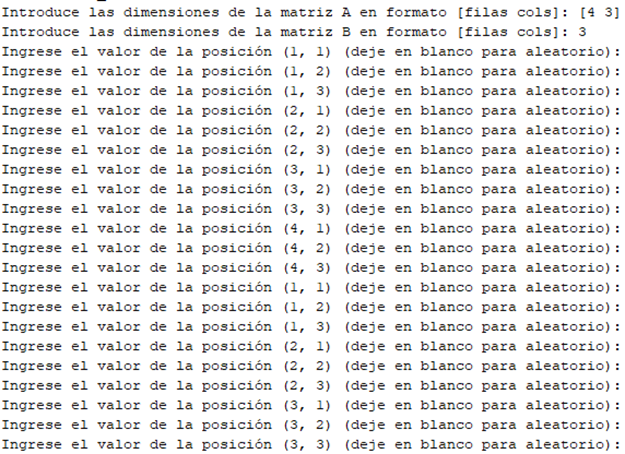
\includegraphics[width=\textwidth]{figures/ejc3.1.png}
			\label{grafica5.1}
		\end{subfigure}
		\begin{subfigure}{0.49\textwidth}
			\centering
			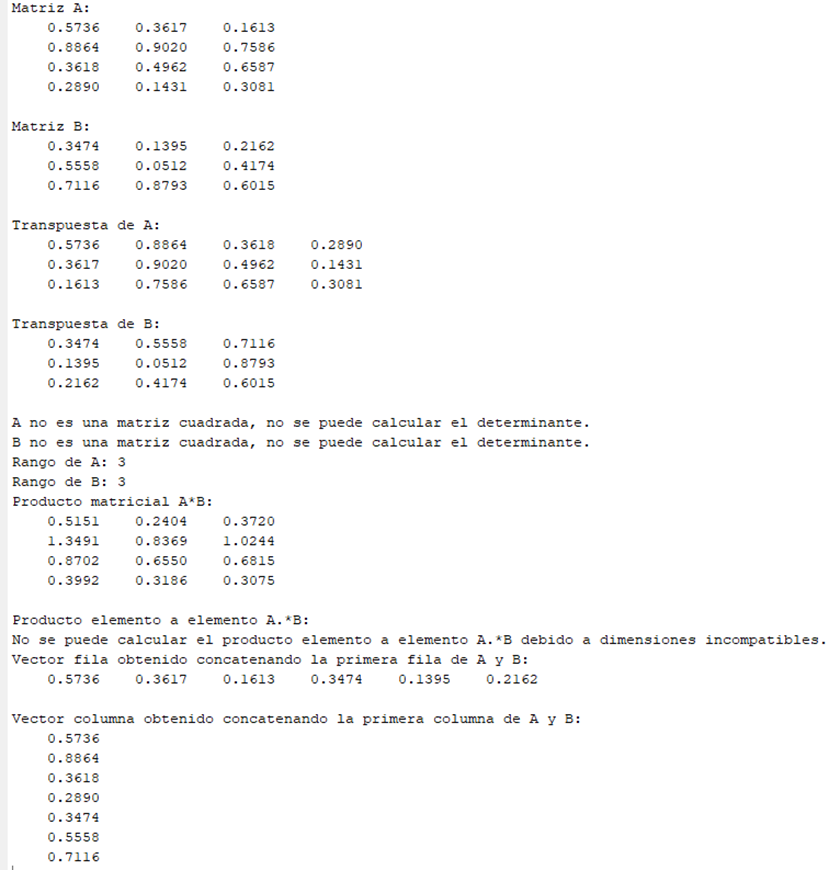
\includegraphics[width=\textwidth]{figures/ejc3.2.png}
			\label{grafica5.2}
		\end{subfigure}
		\caption{Ejecución ejercicio 3.}
		\label{ejec3}
	\end{figure}
	\newpage
	\section{Ejercicio 4. Tiempo de cómputo y representación gráfica.}
	
	\subsection{Código}
	\inputminted[fontsize=\scriptsize, linenos, breaklines=true, xleftmargin=0.75cm, frame=lines]{matlab}{code/Ejercicio4.m}
	\subsection{Ejecución}
	\begin{figure}[htp!]
		\centering
		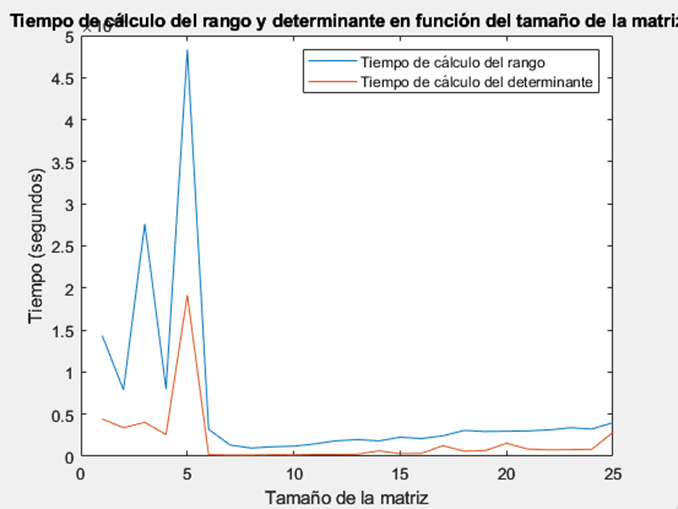
\includegraphics[width=0.6\textwidth]{figures/graf4.png}
		\caption{Gráfico ejecución ejercicio 4.}
	\end{figure}
	
	\section{Ejercicio 5. Representación gráfica en 3D.}
	
	\subsection{Código}
	\inputminted[fontsize=\scriptsize, linenos, breaklines=true, xleftmargin=0.75cm, frame=lines]{matlab}{code/Ejercicio5.m}
	\subsection{Ejecución}
	\begin{figure}[ht]
		\begin{subfigure}{0.49\textwidth}
			\centering
			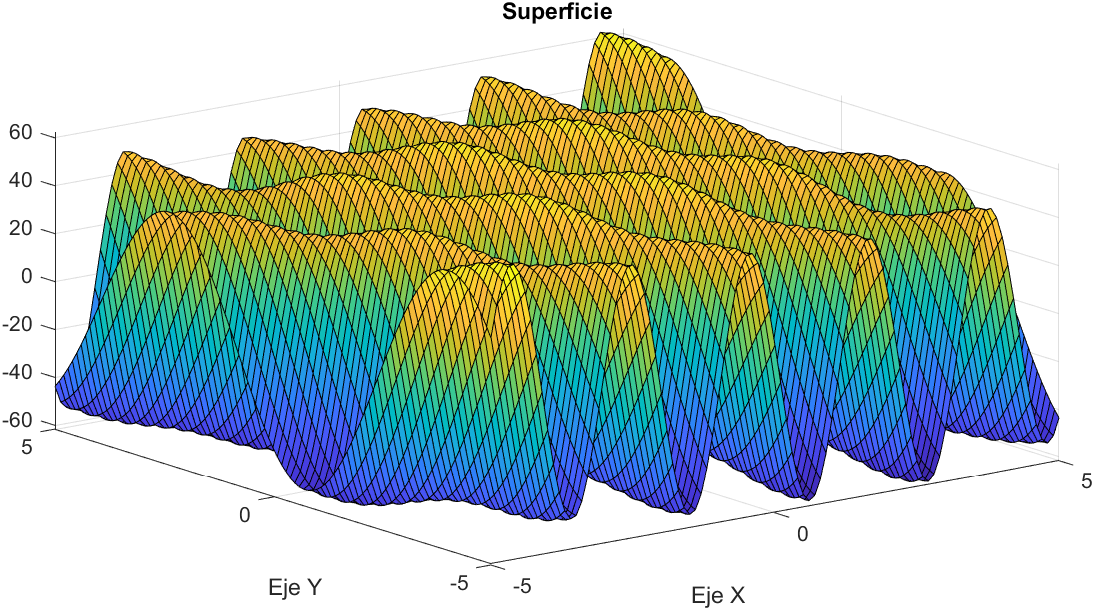
\includegraphics[width=\textwidth]{figures/graf5.1.png}
			\caption{Gráfico de superficie.}
			\label{grafica5.1}
		\end{subfigure}
		\begin{subfigure}{0.49\textwidth}
			\centering
			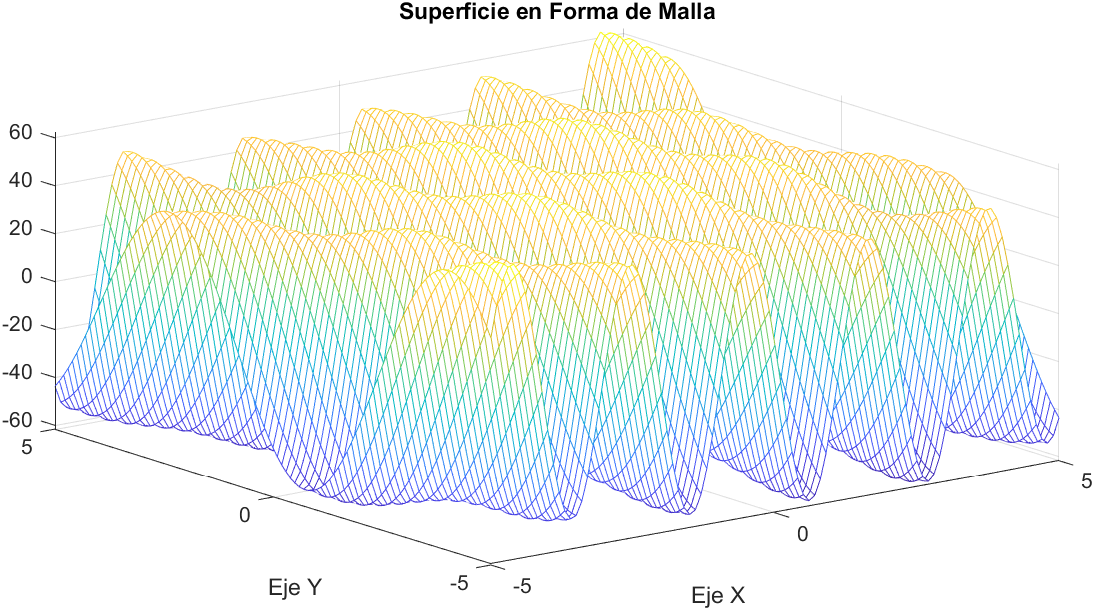
\includegraphics[width=\textwidth]{figures/graf5.2.png}
			\caption{Gráfico de superficie en forma de malla.}
			\label{grafica5.2}
		\end{subfigure}
		\begin{subfigure}{0.49\textwidth}
			\centering
			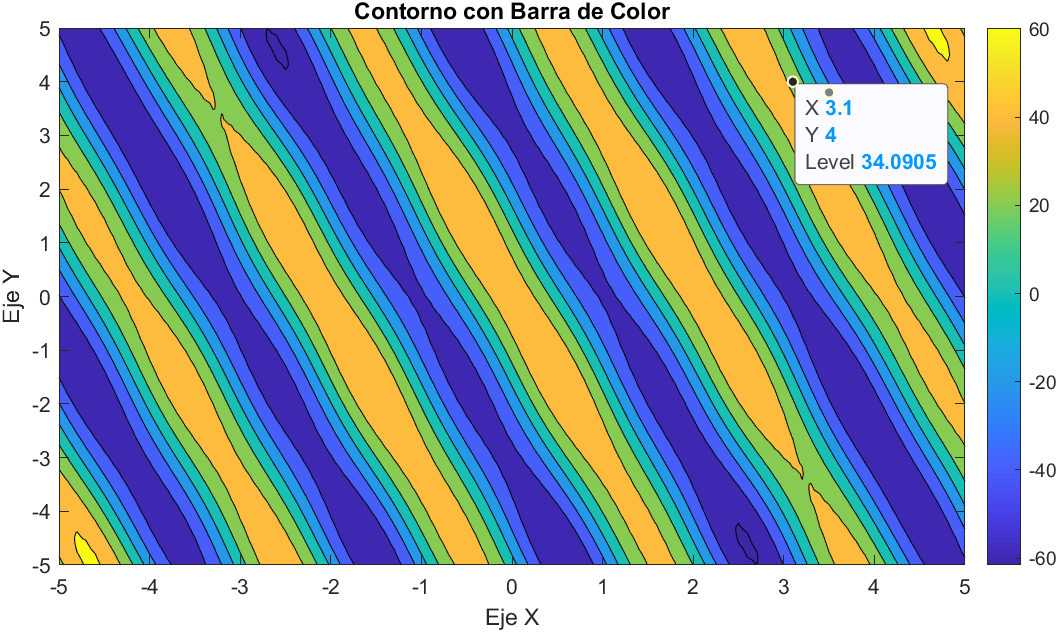
\includegraphics[width=\textwidth]{figures/graf5.3.png}
			\caption{Gráfico de contorno con barra de color.}
			\label{grafica5.3}
		\end{subfigure}
		\caption{Gráficos ejecución ejercicio 5.}
		\label{graficos5}
	\end{figure}
	
	\section{Ejercicio 6. Sistemas lineales.}
	
	\subsection{Código}
	\inputminted[fontsize=\scriptsize, linenos, breaklines=true, xleftmargin=0.75cm, frame=lines]{matlab}{code/Ejercicio6.m}
	\subsection{Ejecución}
	\begin{figure}[htp!]
		\centering
		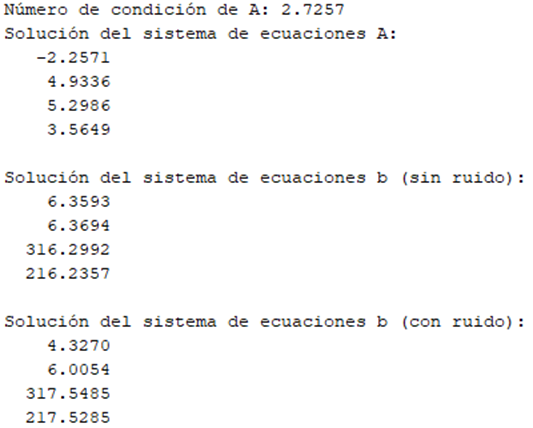
\includegraphics[width=0.6\textwidth]{figures/ejc6.png}
		\caption{Gráfico ejecución ejercicio 6.}
	\end{figure}
	
	\section{Ejercicio 7. Polinomios.}
	
	\subsection{Código}
	\subsubsection*{raices.m}
	\inputminted[fontsize=\scriptsize, linenos, breaklines=true, xleftmargin=0.75cm, frame=lines]{matlab}{code/raices.m}
	\inputminted[fontsize=\scriptsize, linenos, breaklines=true, xleftmargin=0.75cm, frame=lines]{matlab}{code/Ejercicio7.m}
	\subsection{Ejecución}
	\begin{figure}[ht]
		\centering
		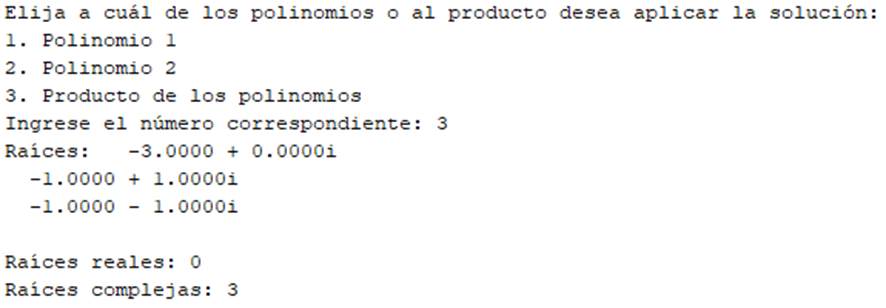
\includegraphics[width=0.6\textwidth]{figures/ejc7.png}
		\caption{Ejecución ejercicio 7.}
		\label{ejec7}
	\end{figure}
	\begin{figure}[ht]
		\centering
		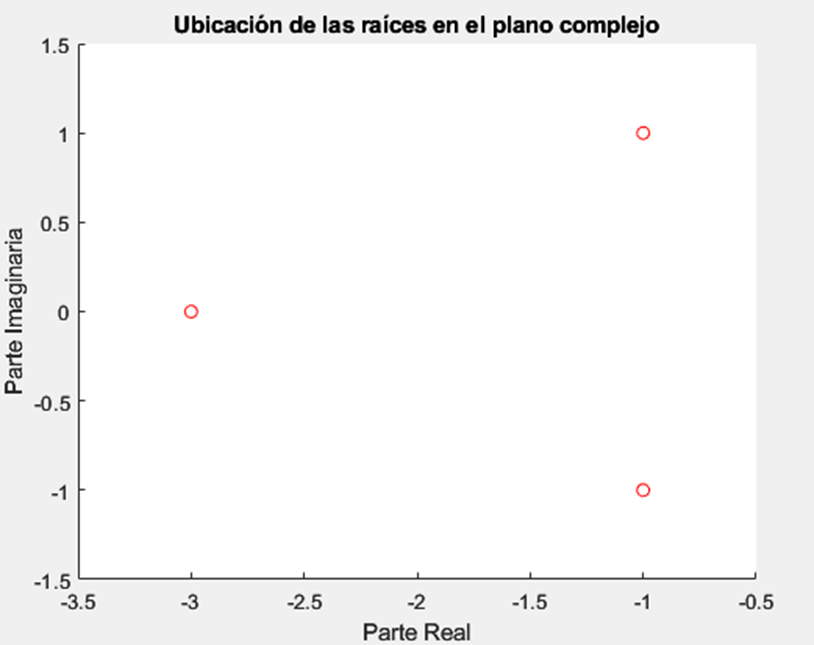
\includegraphics[width=0.5\textwidth]{figures/graf7.png}
		\caption{Gráfico ejecución ejercicio 7.}
		\label{grafica7}
	\end{figure}
	\newpage
	
	\printbibliography
	
\end{document}